\documentclass[tikz]{standalone}

\usepackage{amsmath}
\usepackage{unicode-math}
\usepackage{mathtools}
\usepackage{derivative}

\setmainfont{Stix Two Text}
\setmathfont{Stix Two Math}

\usetikzlibrary{arrows.meta,fit,positioning}

\renewcommand{\familydefault}{\sfdefault}

% prefix equation numbers with section number
\numberwithin{equation}{section}

\DeclarePairedDelimiter{\ceil}{\lceil}{\rceil}
\DeclarePairedDelimiter{\floor}{\lfloor}{\rfloor}
\DeclarePairedDelimiter{\abs}{\lvert}{\rvert}
\DeclarePairedDelimiter{\norm}{\lVert}{\rVert}
\DeclarePairedDelimiter{\bra}{\langle}{\rvert}
\DeclarePairedDelimiter{\ket}{\lvert}{\rangle}
\DeclarePairedDelimiter{\expval}{\langle}{\rangle}
\DeclarePairedDelimiter{\norder}{\mathcolon}{\mathcolon}
\DeclarePairedDelimiter{\anorder}{\typecolon}{\typecolon}
	
\newcommand{\laplace}{\mbfnabla^2}
\newcommand{\trans}{{\scriptscriptstyle\mathsf{T}}}

\newcommand{\vdot}{\cdot}
\newcommand{\vcross}{\vectimes}
\newcommand{\vb}[1]{\symbfup{#1}}
\newcommand{\vu}[1]{\hat{\vb{#1}}}
\newcommand*\dd[2][\relax]{\mathop{\ifx\relax#1\odif{#2}\else \odif[order={#1}]{#2}\fi\,}}

\newcommand{\vacuum}{\ket*{\vb{0}}}

\DeclareMathOperator{\trace}{Tr}
\DeclareMathOperator{\sinc}{sinc}

\AtBeginDocument{
	\let\Re\relax
	\let\Im\relax
	\DeclareMathOperator{\Re}{Re}
	\DeclareMathOperator{\Im}{Im}

	\renewcommand{\div}{\mathop{\mbfnabla\vdot}}
	\newcommand{\curl}{\mathop{\mbfnabla\vectimes}}
}

\DeclarePairedDelimiterX{\comm}[2]{[}{]}{#1,#2}

\DeclarePairedDelimiterX{\braket}[2]{\langle}{\rangle}{#1\delimsize\vert#2}
\DeclarePairedDelimiterX{\ketbra}[1]{\lvert}{\rvert}{#1\rangle\delimsize\langle#1}



\begin{document}
    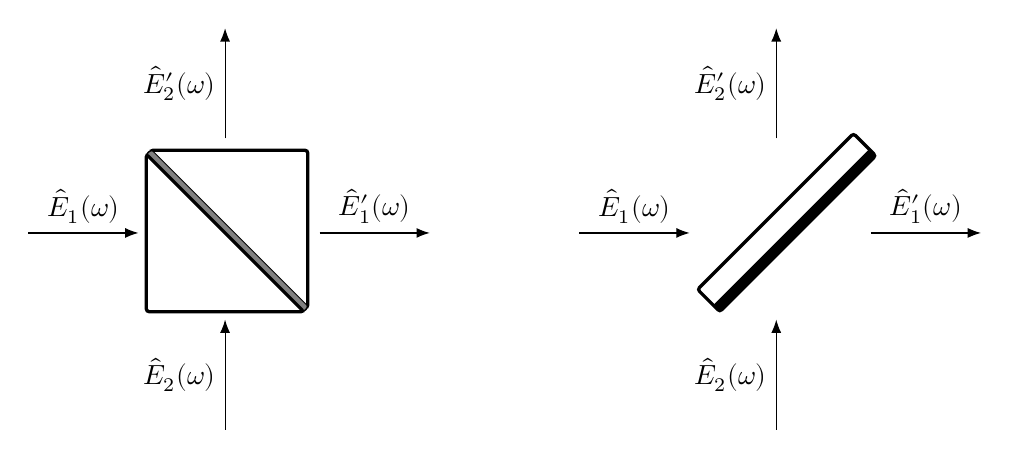
\begin{tikzpicture}
        \begin{scope}
            \coordinate (prism1 a) at (0, 0);
            \coordinate (prism1 b) at (2, 0);
            \coordinate (prism1 c) at (0, 2);
            \draw[very thick] (prism1 b) ++(0.05, 0.05) coordinate (prism2 a);
            \draw[very thick] (prism1 c) ++(0.05, 0.05) coordinate (prism2 c);
            \draw[very thick, rounded corners=1] (prism2 a) -- ++(0, 2) coordinate (prism2 b) -- (prism2 c) -- cycle;
            \filldraw[gray, rounded corners=1] (prism1 b) -- (prism2 a) -- (prism2 c) -- (prism1 c) -- cycle;
            \draw[very thick, rounded corners=1] (prism1 a) -- (prism1 b) -- (prism1 c) -- cycle;
            \draw[very thick, line width=0.5, rounded corners=1] (prism1 a) -- (prism1 b) -- (prism2 a) -- (prism2 b) -- (prism2 c) -- (prism1 c) -- cycle;

            \draw[-Latex] (-1.5,1) -- +(1.4,0) node[midway, above] {$\hat{E}_1(\omega)$};
            \draw[-Latex] (2.2,1) -- +(1.4,0) node[midway, above] {$\hat{E}_1^\prime(\omega)$};
            \draw[-Latex] (1,-1.5) -- +(0,1.4) node[midway, left] {$\hat{E}_2(\omega)$};
            \draw[-Latex] (1,2.2) -- +(0,1.4) node[midway, left] {$\hat{E}_2^\prime(\omega)$};
        \end{scope}

        \begin{scope}[xshift=7cm]
            \begin{scope}[rotate=-45, xshift=-0.2cm, yshift=0.2cm]
                \draw[very thick, rounded corners=1] (0, 0) rectangle (0.4, 2.8);
                \filldraw[black] (0.29, 0) rectangle (0.4, 2.8);
            \end{scope}

            \draw[-Latex] (-1.5,1) -- +(1.4,0) node[midway, above] {$\hat{E}_1(\omega)$};
            \draw[-Latex] (2.2,1) -- +(1.4,0) node[midway, above] {$\hat{E}_1^\prime(\omega)$};
            \draw[-Latex] (1,-1.5) -- +(0,1.4) node[midway, left] {$\hat{E}_2(\omega)$};
            \draw[-Latex] (1,2.2) -- +(0,1.4) node[midway, left] {$\hat{E}_2^\prime(\omega)$};        \end{scope}
    \end{tikzpicture}
\end{document}
